% 2010 年湖北卷理科第 1 题：复平面内的点 E、F、G、H、Z。
% 来源 PDF：普通高考/2010/2010湖北理.pdf，SHA-256 2cfb3d100d55f89c58fe4475caf29f039496afbd0f16d7a7d07857eed5759f55。
% 原页：第 1 页（A3 三栏）第 1 栏上部，书页码 597。
% 重绘依据：按 600 dpi 原页量得虚线网格为 x=-3…3、y=-2…2（每格 1 单位），
%   E(1,2)、Z(3,1)、F(-3,1)、G(-2,-1)、H(2,-1)，与源图点位一致；
%   源图中 E 的点落在 y=2 的网格线上，F、Z 落在 y=1 的网格线上，G、H 落在 y=-1 的网格线上。
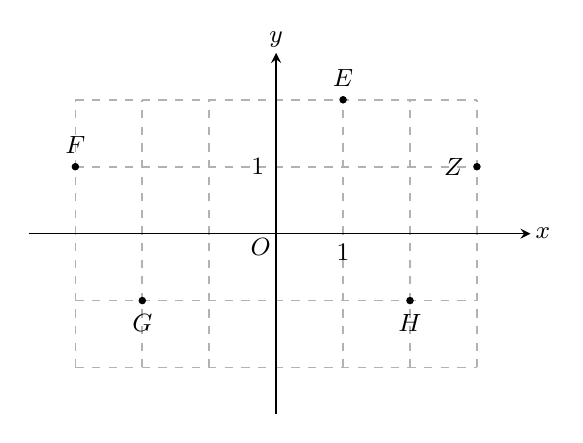
\begin{tikzpicture}[scale=0.85, semithick, every node/.style={inner sep=1.6pt, font=\small}]
  % 虚线网格
  \draw[gray!60, dashed] (-3,-2) grid (3,2);
  % 坐标轴
  \draw[-stealth] (-3.7,0) -- (3.8,0) node[right] {$x$};
  \draw[-stealth] (0,-2.7) -- (0,2.7) node[above] {$y$};
  % 单位标注
  \node[below] at (1,-0.08) {$1$};
  \node[left] at (-0.1,1) {$1$};
  \node[below left] at (0,0) {$O$};
  % 各点
  \fill (1,2) circle (1.6pt) node[above=3pt] {$E$};
  \fill (3,1) circle (1.6pt) node[left=3pt] {$Z$};
  \fill (-3,1) circle (1.6pt) node[above=3pt] {$F$};
  \fill (-2,-1) circle (1.6pt) node[below=3pt] {$G$};
  \fill (2,-1) circle (1.6pt) node[below=3pt] {$H$};
\end{tikzpicture}
